%
% File acl2012.tex
%
% Contact: Maggie Li (cswjli@comp.polyu.edu.hk), Michael White (mwhite@ling.osu.edu)
%%
%% Based on the style files for ACL2008 by Joakim Nivre and Noah Smith
%% and that of ACL2010 by Jing-Shin Chang and Philipp Koehn


\documentclass[11pt,letterpaper]{article}
\usepackage[letterpaper]{geometry}
\usepackage{acl2012}
\usepackage{times}
\usepackage{latexsym}
\usepackage{amsmath}
\usepackage{multirow}
\usepackage{url}
\usepackage{xspace}
\usepackage{paralist}
\usepackage{booktabs}
\usepackage[pdftex]{graphicx}
\makeatletter
\newcommand{\@BIBLABEL}{\@emptybiblabel}
\newcommand{\@emptybiblabel}[1]{}
\makeatother
\usepackage[hidelinks]{hyperref}
\DeclareMathOperator*{\argmax}{arg\,max}
\setlength\titlebox{6.5cm}    % Expanding the titlebox

\def \eg {e.g.,\@ }
\def \ie {i.e.,\@ }
\def \al {al.\@ }
\def \etc {etc.\@ }


\newcommand\BibTeX{B{\sc ib}\TeX}

% TJB macros
\newcommand{\dotts}{...}
\newcommand{\gap}{$*$\xspace}
\newcommand{\z}{\phantom{0}}
\newcommand{\ex}[1]{\textit{#1}\xspace}
\newcommand{\termdef}[1]{\textbf{#1}\xspace}
\newcommand{\termemph}[1]{\textit{#1}\xspace}

\newcommand{\LPR}{\ensuremath{\text{LPR}}}
\newcommand{\minLPR}{\ensuremath{\text{minLPR}}}
\newcommand{\cover}{\ensuremath{\text{cover}}\xspace}
\newcommand{\clear}{\ensuremath{\text{clear}}\xspace}
\newcommand{\overlap}{\ensuremath{\text{overlap}}\xspace}

\newcommand{\figref}[2][]{Figure#1~\ref{#2}\xspace}
\newcommand{\tabref}[2][]{Table#1~\ref{#2}\xspace}
\newcommand{\secref}[2][]{Section#1~\ref{#2}\xspace}



\title{Unsupervised Acquisition of Comprehensive Multiword Lexicons \\ using Competition in an $n$-gram Lattice}

\author{First Author \\
  Affiliation / Address line 1 \\
  Affiliation / Address line 2 \\
  Affiliation / Address line 3 \\
  {\tt email@domain} \\\And
  Second Author \\
  Affiliation / Address line 1 \\
  Affiliation / Address line 2 \\
  Affiliation / Address line 3 \\
  {\tt email@domain} \\}

\date{}

\begin{document}
\maketitle


\begin{abstract}
We present a new model for acquiring comprehensive multiword lexicons from large corpora based on  competition among $n$-gram candidates. In contrast to the standard approach of simple ranking by association measure, in our model $n$-grams are arranged in a lattice structure based on subsumption and overlap relationships, with nodes inhibiting other nodes in their vicinity when they are selected as a lexical item. We show how the configuration of such a lattice can be optimized tractably, and demonstrate using annotations of sampled $n$-grams that our method consistently outperforms alternatives by at least 0.05 F-score across several corpora and languages.
\end{abstract}


\section{Introduction}

Despite over 25 years of research in computational linguistics aimed at acquiring multiword lexicons using corpora statistics, and growing evidence that speakers process language primarily in terms of memorized sequences \cite{Wray08}, the individual word nonetheless stubbornly remains the \textit{de facto} standard processing unit for most research in modern NLP. The potential of multiword knowledge to improve both the automatic processing of language as well as offer new understanding of human acquisition and usage of language is the primary motivator of this work. We present an effective, expandable, and above all tractable new approach to comprehensive multiword lexicon acquisition that aims to find a middle ground between standard MWE acquisition approaches based on association measures \cite{Ramisch14}, and more sophisticated statistical models \cite{Newman12} which fail to scale to the large corpora which are the main sources of the distributional information in modern NLP systems.


%Methods based on association measures tend to assume a small, fixed set of part-of-speech (``POS'') combinations with higher productivity \cite{Evert:Krenn:2001,Pecina10} as a means of reducing overgeneration, with the obvious disadvantage of impeding the generation of a broad-coverage multiword lexicon. This is the central challenge addressed in this paper: how to avoid redundancy/computational intractability when selecting a lexicon from a huge collection of $n$-grams, many of which show basic statistical irregularities only as a result of their syntactic properties or because of partial correspondence with a true multiword lexical item. Our solution to this challenge takes the form of an iterative model, where $n$-gram types compete with each other in a lattice to generate a compact, parsimonious vocabulary which best explains the statistics extracted from the corpus. 

A central challenge in building comprehensive multiword lexicons is pairing down the huge space of possibilities without imposing restrictions which disregard a major portion of the multiword vocabulary of a language: allowing for diversity creates significant redundancy among statistically promising candidates. The lattice model proposed here addresses this primarily by having the candidates---contiguous and non-contiguous $n$-gram types---compete with each other based on subsumption and overlap relations to be selected as the best (\ie most parsimonious) explanation for statistical irregularities due to lexical affinity. We test this approach across four large corpora in three languages, including two relatively free-word-order languages (Croatian and Japanese), and find that this approach consistency outperforms alternatives, offering scalability and many avenues for future enhancement.




\section{Background and Related Work}

In this paper we will refer to the targets of our lexicon creation efforts as \termdef{formulaic sequences}, following the terminology of Wray \shortcite{Wray02,Wray08}, wherein a formulaic sequence (FS) is defined as ``a sequence, continuous or discontinuous, of words or other elements, which is, or appears to be, prefabricated: that is, stored and retrieved whole from memory at the time of use, rather than being subject to generation or analysis by the language grammar.'' That is, a FS shows signs of being part of a mental lexicon. Though by this definition individuals or small groups may have their own FS, here we are only interested in FS that are shared by a recognizable language community. 

In computational linguistics, the most common term used to describe multiword lexical units is \emph{multiword expression} (``MWE'': \newcite{Sag02}, \newcite{Baldwin10}), but here we wish to make a principled distinction between at least somewhat non-compositional, strongly lexicalized MWEs and FS, a near superset which includes many MWEs but also compositional linguistic formulas. This distinction is not a new one; it exists, for example, in the original paper of \newcite{Sag02} in the distinction between lexicalized and institutionalized phrases, and also to some extent in the MWE annotation of \newcite{Schneider14a}, who distinguish between weak (collocational)\footnote{Here we avoid the term \emph{collocation} entirely due to confusion with respect to its interpretation. Though some define it similarly to our definition of FS, it can be applied to any words that show a statistical tendency to appear in the vicinity of one another for any reason: for instance, the pair of words \ex{doctor/nurse} might be considered a collocation \cite{Ramisch14}.}  and strong (non-compositional) MWEs. It is our contention, however, that separate, precise terminology is useful for research targeted at either class: we need not strain the concept of MWE to include items which do not require special semantics, nor are we inclined to disregard the larger formulaticity of language simply because it is not the dominant focus of MWE research. Many MWE researchers might defensibly balk at including in their MWE lexicons and corpus annotations (English) FS such as \ex{there is something going on}, \ex{it is more important than ever to \dotts}, \ex{\dotts do not know what it is like to \dotts}, \ex{there is no shortage of\dotts}, \ex{the rise and fall of\dotts}, \ex{now is not the time to\dotts}, \etc as well as tens of thousands of other such phrases which, along with less compositional MWEs like \ex{be worth \dotts's weight in gold}, fall under the FS umbrella. Another reason to introduce a different terminology is that there are classes of what is typically considered MWE that do not fit well into an FS framework, for instance novel compound nouns whose semantics are accessible by analogy (\eg \ex{glass limb} or \ex{government ambiguity}). Also, we exclude from the definition of both FS and MWE those named entities which refer to people or places which are little-known and/or whose surface form appears derived (\eg \ex{Mrs.\ Barbara W.\ Smith} or \ex{Smith Garden Supplies Ltd}). \figref{fig:terminology} shows the conception of the relationship between FS, MWE, and (multiword) named entities that we assume for this paper.


\begin{figure}[!t]
\center{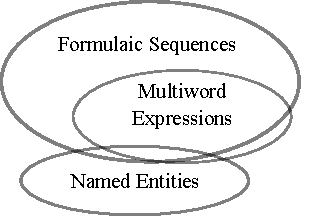
\includegraphics[width=0.3\textwidth]{FS_diagram_1.pdf}}
\caption{Multiword Terminology}
\label{fig:terminology}
\end{figure}



Regardless of the terminology used to describe them, the starting point for multiword lexicon creation has typically been lexical association measures \cite{Church90,Dunning93,Schone01,Evert04,Pecina10,DeAraujo11,Kulkarni11,Ramisch14}. When these methods are used to build a lexicon, particular binary syntactic patterns are typically chosen. Only some of these measures generalize tractably beyond two words, for example PMI \cite{Church90}, i.e., the log ratio of the joint probability to the product of the marginal probabilities of the individual words. Other measures specifically designed to address sequences of larger than two words include: the $c$-value \cite{Frantzi00}, a metric designed for term extraction which weights term frequency by the log length of the $n$-gram while penalizing $n$-grams that appear in frequent larger ones; and mutual expectation \cite{Dias99}, which produces a normalized statistic that reflects how much a candidate phrase resists the omission of any particular word. Similarly, the lexical predictability ratio (LPR) of \newcite{Brooke15b} is an association measure intended for any possible syntactic pattern which is calculated by discounting syntactic predictability from the overall conditional probability for each word given the other words in the phrase. Though most association measures involve only usage statistics of the phrase and its subparts, the DRUID measure is an exception which uses distributional semantics around the phrase to identify how easily an $n$-gram could be replaced by a single word \cite{Riedl15}.

Typically multiword lexicons are created by ranking $n$-grams according to an association measure and applying a threshold. The algorithm of \newcite{Silva99} is somewhat more sophisticated, in that it identifies the local maxima of association measures across subsuming $n$-grams within a sentence to identify MWEs of unrestricted length and syntactic composition; its effectiveness beyond noun phrases, however, seems relatively limited \cite{Ramisch12}. Brooke et \al \shortcite{Brooke14a,Brooke15b} developed a heuristic method intended for general FS extraction in larger corpora, first using conditional probably statistics to do an initial (single pass) coarse-grained segmentation of the corpus, followed by a pass through the resulting vocabulary, breaking larger units into smaller ones based on a tradeoff between marginal and conditional statistics. Beyond association measures, other general unsupervised approaches to the multiword unit identification include that of \newcite{Newman12}, who used a generative Dirichlet Process model which jointly creates a linear segmentation of the corpus and a multiword vocabulary of keyphrases.

Other research in MWEs has tended to be rather focused on particular syntactic patterns such as verb-noun combinations \cite{Fazly09}. The work of \newcite{Schneider14b} is a rare example of a comprehensive token-level MWE identification system which distinguishes a full range of MWE sequences in the English Web Treebank, including those involving gaps, using a supervised sequence tagging model. Schneider et \al make use of existing manual lexical resources and note that an (unsupervised) automatic lexical resource could be useful addition to the model, although attempts to do so have achieved mixed success \cite{Riedl16}. 

The motivation for building lexicons of FS naturally overlaps with those for MWE: models of distributional semantics, in particular, can benefit from sensitivity to multiword units \cite{Cohen:Widdows:2009}, as can parsing \cite{Constant16} and topic models \cite{Lau+:2012b}. One major motivation for looking beyond MWEs is the ability to carry out broader linguistic analyses. Within corpus linguistics, multiword sequences have been studied in the form of \textit{lexical bundles} \cite{Biber04}, which are simply $n$-grams that occur above a certain frequency threshold. Like FS, Lexical bundles generally involve larger phrasal chunks that would be missed by traditional MWE extraction, and so research in this area has tended to focus on how particular formulaic phrases (\eg \textit{if you look at}) are indicative of particular genres (\eg university lectures). Lexical bundles have been applied, in particular, to learner language: for example,  \newcite{Chen10} show that non-native student writers use a severely restricted range of lexical bundle types, and tend to overuse those types, while \newcite{Granger14} investigate the role of proficiency, demonstrating that intermediate learners underuse lower-frequency bigrams and overuse high-frequency bigrams relative to advanced learners. \newcite{Sakaguchi16} demonstrate that improving fluency (closely linked to the use of linguistic formulas) is more important than improving strict grammaticality with respect to native speaker judgments of non-native productions; \newcite{Brooke15b} explicitly argue for FS lexicons as a way to identify, track, and improve learner proficiency.


\section{Method}

Our approach to FS identification involves optimization of the total explanatory power of a lattice, where each node corresponds to an $n$-gram type. The explanatory power of the whole lattice is defined simply as a product of the \termdef{explainedness} of the individual nodes. Each node can be considered either ``on'' (is an FS) or ``off'' (is not an FS). The basis of the calculation of explainedness is the syntax-sensitive LPR association measure of \newcite{Brooke15b}, but it is calculated differently depending on the on/off status of the node as well as the status of the nodes in the vicinity: nodes are linked based on $n$-gram subsumption and corpus overlap relationships (see \figref{fig:example}), with ``on'' nodes typically explaining other nodes.  Given these relationships, we iterate over the nodes and greedily optimize the on/off choice relative to explainedness in the local neighborhood of each node, until convergence.

\subsection{Collecting statistics}

The first step in the process is to derive a set of $n$-grams and related statistics from a large, unlabeled corpus of text. Since our primary association measure is an adaption of LPR, our approach in this section mostly follows \newcite{Brooke15b} up until the last stage. An initial requirement of any such method is an $n$-gram frequency threshold, which we set to 1 instance per 10 million words, following \newcite{Brooke15b}.\footnote{Based on manual analysis using the MWE corpus of \newcite{Schneider14a}, this achieves very good (over 90\%) type-level MWE coverage using the frequency filtered $n$-gram statistics from the ICWSM blog corpus (see \secref{sec:evaluation}) after filtering out proper names.} 

We include gapped or non-contiguous $n$-grams in our analysis, in acknowledgment of the fact that many languages have MWEs where the components can be ``separated'', including verb particle constructions in English \cite{Dehe:2002}, and noun--verb idioms in Japanese \cite{Hashimoto:Kawahara:2008}. Having said this, there are generally strong syntactic and length \cite{Wasow:2002} restrictions on what can constitute a gap, which we capture in the form of a language-specific POS-based regular expression (see \secref{sec:evaluation} for details).
This greatly lowers the number of potentially gapped $n$-gram types, increasing precision and efficiency for negligible loss of recall. We also exclude punctuation and lemmatize the corpus, and enforce an $n$-gram count threshold. As long as the count threshold  is substantially above 1, efficient extraction of all $n$-grams can be done iteratively: in iteration $i$, $i$-grams are filtered by the frequency threshold, and then pairs of instances of these $i$-grams with $(i-1)$ words of overlap are found, which derives a set of $(i+1)$-grams which necessarily includes all those over the frequency threshold. 

Once a set of relevant $n$-grams is identified and counted, other statistics required to calculate the \termdef{Lexical Predictability Ratio} (``LPR'') for each word in the $n$-gram are collected. LPR is a measure of how predictable a word is in a lexical context, as compared to how predictable it is given only syntactic context (over the same span of words). Formally, the LPR for word $w_i$ in the context of a word sequence $w_1,..., w_i, ..., w_{n}$ with POS tag sequence $t_1, ..., t_{n}$, is given by:
\begin{displaymath}
\LPR(w_i,w_{1,n}) = \max_{1 \leq j < k \leq n }{\frac{p(w_i|w_{j,k})}{p(w_i|t_{j,k})}}
\end{displaymath}
where $w_{j,k}$ denotes the word sequence $w_j,..., w_{i-1}, w_{i+1}, ..., w_{k}$ excluding $w_{i}$ (similarly for $t_{j,k}$). Note that the lower bound of LPR is 1, since the ratio for a word with no context is trivially 1. We use the same equation for gapped $n$-grams, with the caveat that quantities involving sequences which include the location where the gap occurs are derived from special gapped $n$-gram statistics. %Note that the identification of the best ratio across all possible choices of context, not just the largest, is important for longer FS, where the entire POS context alone might uniquely identify the phrase, resulting in the minimum LPR of 1 even for entirely formulaic sequences, an undesirable result. 


In the segmentation approach of \newcite{Brooke15b}, LPR for an entire span is calculated as a product of the individual LPRs, but here we will use the minimum LPR across the words in the sequence:
\begin{displaymath}
\minLPR(w_{1,n}) = \min_{1 \leq i \leq n }{\LPR(w_i,w_{1,n})}
\end{displaymath}
Here, minLPR for a particular $n$-gram does not reflect the \emph{overall} degree to which it holds together, but rather focuses on the word which is its weakest link. For example, in the case of \ex{be keep \gap under}, a general statistical metric might assign it a high score due to the strong association between \ex{keep} and \ex{under}, but minLPR is focused on the weaker relationship between \ex{be} and \ex{keep \gap under}.


\begin{figure}[!tb]
\center{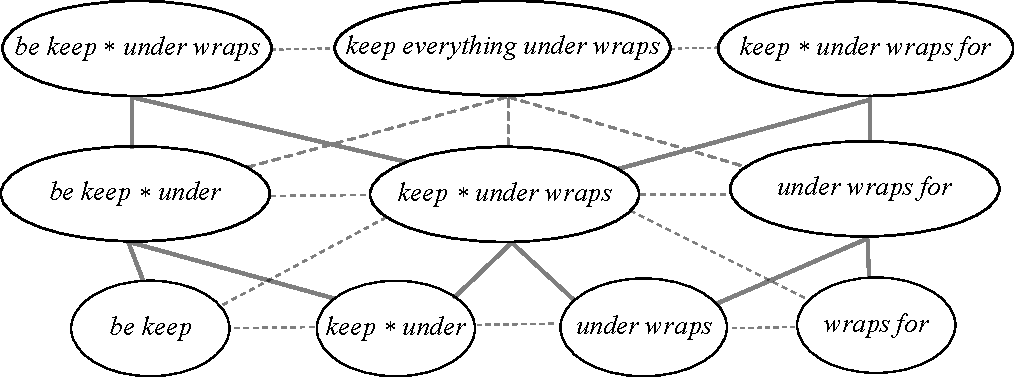
\includegraphics[width=0.5\textwidth]{FS_diagram_2.pdf}}
\caption{A portion of an $n$-gram lattice. Solid lines indicate subsumption, dotted lines overlaps}
\label{fig:example}
\end{figure}

\subsection{Node interactions}

The $n$-gram nodes in the lattice are directionally connected to nodes consisting of $(n+1)$-grams which subsume them and $(n-1)$-grams which they subsume. For example, as detailed in \figref{fig:example}, the (gapped) $n$-gram \ex{keep \gap under wraps} would be connected ``upwards'' to the node \ex{keep everything under wraps} and connected ``downwards'' to \ex{under wraps}. These directional relationships allow for two basic interactions between nodes in the lattice when a node is turned on: \termdef{covering}, which inhibits nodes below (subsumed by) a turned-on node (\eg if \ex{keep \gap under wraps} is on, the model will tend not to choose \ex{under wraps} as an FS); and \termdef{clearing}, which inhibits nodes above a turned-on node (\eg if \ex{keep \gap under wraps} is on, the model would avoid selecting \ex{keep everything under wraps} as an FS). A third, undirected mechanism is \termdef{overlapping}, where nodes inhibit each other due to overlaps in the corpus (\eg having both \ex{keep \gap under wraps} and \ex{be keep \gap under} as FS will be avoided).


\subsubsection{Covering}
The most important node interaction is \termdef{covering}, which corresponds to discounting or entirely excluding a node due to a node higher in the lattice. Our model includes two types of covering: hard and soft. 

\termdef{Hard covering} is based on the idea that, due to very similar counts, we can reasonably conclude that the presence of an $n$-gram in our statistics is a direct result of the other. In \figref{fig:example}, \eg if we have 143 counts of \ex{keep \gap under wraps} and 152 counts of \ex{under wraps}, the presence of \ex{keep \gap under wraps} almost completely explains \ex{under wraps}, and we should consider these two $n$-grams as one. We do this by permanently disabling any hard covered node, and setting the minLPR of the covering node to the maximum minLPR among all the nodes it covers (including itself); this means that longer $n$-grams with function words (which often have lower minLPR) can benefit from the strong statistical relationships between open-class lexical features in $n$-grams that they cover. This is done as a preprocessing step, and greatly improves the tractability of the iterative optimization of the lattice. Of course, a threshold for hard covering must be chosen: empirically, we have found that a ratio of $2/3$ (corresponding to a significant majority of the counts of a lower node corresponding to the higher node) works well.  We also use the concept of hard covering to address the issue of pronouns, based on the observation that pronouns often have high LPR values \cite{Brooke15b}. In the lattice, $n$-grams with pronouns are considered covered (inactive) unless they cover at least one other node which does not have a pronoun, which allows us to limit FS with pronouns without excluding them entirely: they are included only in cases where they are definitively formulaic. 

\termdef{Soft covering} is used in cases when a single $n$-gram does not entirely account for another, but a turned-on $n$-gram to some extent may explain some of the statistical irregularity of one lower in the lattice. For instance, in \figref{fig:example} \ex{keep \gap under} is not hard-covered by \ex{keep \gap under wraps} (since there are FS such as \ex{keep \gap under surveillance}, \ex{keep it under your hat}, \etc), but if \ex{keep \gap under wraps} is tagged as an FS, we nevertheless want to discount the portion of the \ex{keep \gap under} counts that correspond to occurrences of \ex{keep \gap under wraps}. This is accomplished by increasing the turned-off explainedness of \ex{keep \gap under} (and thus making turning on less desirable) in the following manner: let $c(\cdot)$ be the count function, and $s_1\dotts s_m$ be any turned-on nodes which are above $t$ in the lattice (covering nodes). Then, the $\cover(t)$ score for a covered node $t$ is:
\begin{displaymath}
\cover(t) = \max\Big(0,\frac{c(t) - \sum_{i=1}^{m}{c(s_i)}}{c(t)}\Big)
\end{displaymath}
This is intended as a simple, quick-to-calculate approximation of the result of recalculating minLPR with the counts corresponding to the covering nodes actually removed. \cover takes on values in the range 0 to 1, with 1 being the default when no covering is occurring.

\subsubsection{Clearing}

In general, covering prefers turning on longer, covering $n$-grams since doing so explains nodes lower in the lattice. Not surprisingly, it is generally desirable to have a mechanism working in opposition, \ie one which views shorter FS as helping to explain the presence of longer $n$-grams which contain them, beyond the FS-neutral syntactic explanation provided by minLPR. \termdef{Clearing} does this by changing the $E_0$ of nodes higher in the lattice when a lower node is turned-on. The basic mechanism is similar to covering, except that counts cannot be made use of in the same way---whereas it makes sense to explain covered nodes in proportion to the counts of their covering nodes (since the counts of the covered $n$-grams are from the covering $n$-gram), in the reverse direction this logic fails. 

A simple but effective solution which avoids introducing extra hyperparameters is to make use of the minLPR values of the relevant nodes. In the most common two-node situation, we increase the explainedness of the cleared node based on the ratio of the minLPR of two nodes, though only if the minLPR of the lower node is higher. Generalized to the (rare) case of multiple clearing nodes, we define $\clear(t)$ as:
%in this paper, we consider two options: a hard clearing where any turned-on node will clear (set $C_{0}$ to 0 for) any node higher in the lattice which has a minLPR that is lower than it; and a soft 
\begin{displaymath}
\clear(t) = \prod_{i=1}^{m}{\min\Big(1,\frac{\minLPR(t)}{\minLPR(u_i)}\Big)}
\end{displaymath}
where $u_i$ is the $i$th clearing node of $t$, \ie turned-on nodes below $t$ in the lattice. We refer to this mechanism as ``clearing'' because it tends to clear away a variety of trivial uses of common FS which may have higher LPR due to the lexical and syntactic specificity of the FS. For instance, in \figref{fig:example} if the node \ex{keep \gap under wraps}  is turned on and has a minLPR of 8, then, if the minLPR of a node such as \ex{keep \gap under wraps for} is 4, $\clear(t)$ will be 0.5. Like \cover, \clear takes on values in the range 0 to 1, with 1 being the default when no clearing occurs. 

%We can now define $d_{0}(t)$ as:
%\begin{displaymath}
%d_0(t) = \cover(t) \cdot \clear(t)
%\end{displaymath}
%Note that the effect of both covering and clearing is to increase explainedness for covered/cleared nodes, which indirectly encourages the model to turn an $n$-gram like \ex{keep \gap under wraps} on in order to explain nodes in its vicinity, even supposing its minLPR were relatively low.


\subsubsection{Overlap}

The third mechanism of node interaction involves $n$-grams which overlap in the corpus. In general, independent FS do not consistently overlap. For example, given that \ex{be keep \gap under} and \ex{keep \gap under wraps} often appear together (overlapping on the tokens \ex{keep \gap under}), we do not want both being selected as an FS, even in the case that both have high minLPR. To address this problem, we use a mechanism somewhat different than above: rather than increasing the explainedness of turned-off nodes, we decrease the explainedness of the overlapping turned-on nodes---a penalty rather than an incentive which expresses the model's confusion at having overlapping FS. Let $\mathit{oc}(x,y)$ refer to number of times the $n$-grams corresponding to nodes $x$ and $y$ overlapped in the corpus, and $o_1,\dotts,o_m$ refer to overlapping nodes, \ie turned-on nodes which overlap with our target node $t$in the corpus. We define \overlap(t) as:
\begin{displaymath}
	\overlap(t) = \frac{c(t)}{c(t) - \sum_{i=1}^{m}{\mathit{oc}(t,o_i)}}
\end{displaymath}

Overlap takes on values in the range 1 to $+\infty$, also defaulting to 1 when no overlaps exist. The effect of overlap is hyperbolic: small amounts of overlap have little effect, but nodes with significant overlap will effectively be forced to turn off. 

\subsection{Explainedness}

In order to capture the current state of the model and provide an overall explainedness store, we introduce two indicator functions: $I_{on}(t)$ is 1 if $t$ is on and 0 if $t$ is off ; $I_{\mathit{off}}(t)$ is the reverse. The objective function maximized by the model is then the explainedness ($expl$) across all the nodes of the lattice, which can be defined in terms of minLPR and the node interaction functions:

\begin{multline}
expl(t_1,...,t_N) = \prod_{i=1}^{N}{I_{on}(t_i)  C^{-\overlap(t_1)}} \\ + I_{\mathit{off}}(t_i) minLPR(t_i)^{-\cover(t_i) \cdot \clear(t_i)}
\end{multline}

When a node is off, its explainedness is the inverse of its minLPR, except if there are covering or clearing nodes which explain it by pushing the exponent of minLPR towards zero. When the node is on, its explainedness is the inverse of a fixed cost hyperparameter C, though this cost is increased if it overlaps with other active nodes. 
All else being equal, when $\minLPR(t) > C$, a node will be selected as an FS, and so, independent of the node interactions, C can be viewed as the threshold for the minLPR association measure under a traditional approach to MWE identification. There is no upper bound on $C$, but empirically, we have found values in the range $[3,6]$ give reasonable results for the languages presented in this paper.


%\subsection{Node explainedness functions}

%The central process of the model is to decide which nodes in an $n$-gram lattice correspond to an FS, based on the objective of maximizing the overall explanatory power of the lattice. Like probabilities, explainedness of individual nodes will vary between 0 and 1, with 1 corresponding to a node which is fully explained. We define the explainedness of a node in terms of two functions, capturing the impact on surrounding nodes of a node being either off or on. When a node is off, it is generally desirable (or at least not undesirable) that connected nodes in the lattice are on, since they may serve to partially or entirely explain its existence. When a node is on, however, the presence of other turned-on nodes nearby suggests redundancy, and is not to be encouraged. 

%Let $E_{1}$ be the explainedness of a node when it is on (corresponding to an $n$-gram which has been identified as an FS), and $E_{0}$ be the explainedness of a node when it is off. We calculate $E_{0}$ based on the inverse of minLPR: 
%\begin{displaymath}
%E_0(t) = \minLPR(t)^{-d_0(t)}
%\end{displaymath}
%and $E_{1}$ based on the inverse of a cost parameter $C$:
%\begin{displaymath}
%E_1(t) = C^{-d_1(t)}
%\end{displaymath}
%where $d_0$ and $d_1$ are non-negative functions which capture the lattice context (when there is no context, both default to 1), as detailed in the next section. When the minLPR metric is 1 (corresponding to the case of the syntactic content predicting one of the words of the $n$-gram as well or better than the lexical context), $E_{0}=1$. $E_1$ is equivalent to the initial threshold for building a vocabulary using the minLPR association measure for nodes not influenced by one of the other factors discussed below: all else being equal, when $\minLPR(t) > C$, a node will be selected as an FS. There is no upper bound on $C$, but empirically, we have found a value in the range $[3,6]$ gives reasonable results for the languages presented in this paper.% we note here that there is a fairly small range of good choices for $C$; we have found that setting it too high ($>6$, corresponding to minimum of six times more likely than predicted by POS context alone) will restrict the model primarily to sequences with only open-class words, while setting it too low ($<3$) results in too much random noise.


% The values of $d_0$ and $d_1$ are dependent on the context of the node in the lattice as discussed in the next section, but are both 1 when a node is not influenced by other nodes.


 
\subsection{Optimization}

The dependence of the explainedness of nodes on their neighbors effectively prohibits a global optimization of the lattice. Fortunately, though most of the nodes in the lattice are part of a single main connected component, most of the effects of nodes on each other are relatively local, and effective local optimizations can be made tractable by applying some simple restrictions. The main optimization loop consists of iterations over the lattice until complete convergence (no changes in the final iteration). For each iteration over the main loop, each potentially active node is examined in order to evaluate whether its current status is optimal given the current state of the lattice. The order that we perform this has an effect on the result: among the obvious options, good results are obtained through ordering nodes by frequency, which gives an implicit advantage to relatively common $n$-grams.

Given the relationships between nodes, it is obviously not sufficient to consider switching only the present node. If, for instance, one or more of \ex{be keep \gap under wraps}, \ex{under wraps}, or \ex{be keep \gap under} has been turned on, the covering, blocking, or overlapping effects of these other nodes will likely prevent a competing node like \ex{keep \gap under wraps} from being correctly activated. Instead, the algorithm identifies a small set of ``relevant'' nodes which are the most important to the status of the node under consideration. Since turned-off nodes have no direct effect on each other, only turned-on nodes above, below, or overlapping with the current node need be considered.  Once the relevant nodes have been identified, all nodes (including turned-off nodes) whose explainedness is affected by one or more of the relevant nodes are identified, and then a greedy search is carried out for the optimal configuration of the relevant nodes, starting from an `all-on' state and at each step turning off the node (if any) which most increases overall explainedness.

In practice, we apply the following efficiency restrictions, which significantly reduce the runtime without sacrificing quality (based on development set testing):
\begin{compactitem}
\item We limit the total number of relevant nodes to 5. When there are more than 5 nodes turned on in the vicinity of the target node, the most relevant nodes are selected by ranking candidates by the change in explainedness across possible configurations of the target and candidate node considered in isolation;
\item To avoid having to deal with storing and processing trivial overlaps, we exclude overlaps with a count of less than 5 from our lattice;
\item Many nodes have a minLPR which is slighlty larger than 1. There is very little chance these nodes will be activated by the algorithm, and so after applying hard covering, we do not consider activating nodes with $\minLPR < 2$.
\end{compactitem}

\section{Evaluation}
\label{sec:evaluation}

We evaluate our approach across three different languages including evaluation sets derived from four different corpora. In English, we follow \newcite{Brooke15b} in using a 890M token filtered portion of the ICWSM blog corpus \cite{ICWSM} tagged with the Tree Tagger \cite{Schmid95}. To facilitate a comparison with \newcite{Newman12}, which does not scale up to a corpus as large as the ICWSM, we also build a lexicon using the 100M token British National Corpus \cite{BNC}, using the standard CLAWS-derived POS tags for the corpus. Lemmatization included removing all inflectional marking from both words and POS tags. For English, gaps are identified using the same POS regex used in \newcite{Brooke15b}, which includes simple nouns and portions thereof, up to a maximum of 4 words.



The other two languages we include in our evaluation are Croatian and Japanese. Relative to English, both languages have freer word order: we were interested in probing the challenges associated with using an $n$-gram approach to FS identification in such languages. For Croatian, we used the fhrWaC corpus \cite{snajder2013building}, a filtered version of the Croatian web corpus hrWaC \cite{ljubesic2014bs}, which is POS-tagged and lemmatized using the tools of \newcite{agic2013lemmatization}. Similar to English, the POS regex for Croatian includes simple nouns, adjectives and pronouns, but also other elements that regularly appear inside FS, including both adverbs and copulas. For Japanese, we used a subset of the 100M-page web corpus of \newcite{Shinzato+:2008}, which was roughly the same size (in terms of token count) as the English corpus. We segmented and POS-tagged the corpus with MeCab \cite{Kudo:2008} using the UNIDIC morphological dictionary \cite{Den:2007}. The POS regex for Japanese covers the same basic nominal structures as English, but also includes case markers and adverbials. Though our processing of Japanese includes basic lemmatization related to superficial elements like the choice of writing script and politeness markers, many elements (such as case marking) which are removed by lemmatization in Croatian are segmented into independent morphological units in the MeCab output, making the task somewhat different for the two languages.

\newcite{Brooke15b} introduced a method for evaluating FS extraction without a reference lexicon or direct annotation of the output of a model. Instead, $n$-grams are sampled after applying the frequency threshold and annotated as being either an FS or not, allowing for calculation of a true F-score for any model. We use the annotation of 2000 $n$-grams in the ICWSM corpus from that earlier work, and applied the same annotation methodology to the other corpora discussed above: after training and based on written guidelines derived from the definitions of \newcite{Wray08}, three native-speaker, educated annotators judged 500 contiguous $n$-grams and another 500 gapped $n$-grams for each of the new corpora. 


%. One advantage of a type-based annotation approach (as compared to a corpus annotation), particularly with regards to an task with a known subjective component, is that it is quite sensible to simply discard borderline cases


\begin{table}[!bt]
 
 \begin{center}
   \begin{tabular}{lc@{\,\,\,}cc@{\,\,\,}c@{\,\,\,}c}

       \toprule
       & \multicolumn{2}{c}{Contiguous} & \multicolumn{2}{c}{Gapped} & \multirow{2}{*}{$\kappa$}\\
       \cmidrule(lr){2-3}\cmidrule(lr){4-5}
			& FS & non-FS & FS & non-FS &  \\
			 \midrule
			ICWSM    & 169  & 702 & 29 & 916 & 0.84 \\
			BNC      & \z49 & 403 & \z8& 475 & 0.84 \\
			Croatian & \z64 & 382 & 11 & 456 & 0.87 \\
			Japanese & 124  & 286 & 36 & 341 & 0.81\\
       \bottomrule
 \end{tabular}
  \caption{ Statistics for test sets }
	 \label{tab:stats}

 \end{center}

 \end{table}

Other than the inclusion of new languages, our test sets differ from \newcite{Brooke15b} in two ways. First, instead of relying on strict majority annotation, we entirely excluded $n$-grams which just one annotator marked as FS, improving the reliability of evaluation at the cost of some representativeness.  Second, for the main evaluation we collapsed gapped and contiguous $n$-grams into a single test set. The rationale is that the number of positive gapped examples was too low (particularly for the BNC and the Croatian corpus) to provide a reliable independent F-score (see further discussion in \secref{sec:discussion}). Statistics for the four test sets are given in \tabref{tab:stats}.



 \begin{table*}[!bt]
 
 \begin{center}
 \begin{tabular}{lcccccccccccccccc}

       \toprule
				& \multicolumn{7}{c}{\bf{English}} \\
       \cmidrule(lr){2-8}			
       & \multicolumn{3}{c}{\bf{ICWSM}} & &  \multicolumn{3}{c}{\bf{BNC}} & & \multicolumn{3}{c}{\bf{Croatian}}  && \multicolumn{3}{c}{\bf{Japanese}} \\
       \cmidrule(lr){2-4} \cmidrule(lr){6-8} \cmidrule(lr){10-12} \cmidrule(lr){14-16}
           \multicolumn{1}{c}{\bf{Source}}    & P & R & F &   & P & R & F &   & P & R & F &  & P & R & F \\
          \midrule 
PMIrank & 0.24& 0.15& 0.18 & & 0.12 & 0.25 & 0.16 & & 0.21 &0.32 & 0.26 & & 0.23& 0.09 & 0.15 \\ 
minLPRrank & 0.49& 0.31 & 0.39 & & 0.25& 0.44 & 0.32 & & 0.36 & 0.45 & 0.40 &  & 0.51 & 0.14 & 0.22 \\ 

LPR-seg  &0.53 & 0.42 & 0.47 && 0.37 & 0.44 & 0.40 & & 0.41 & 0.47  & 0.43 &  & 0.77 & 0.34 & 0.47 \\ 
  \midrule

	Lattice \emph{$-$cl} & 0.57& 0.42 & 0.49 & & 0.33& 0.58 & 0.42 & & 0.39 & 0.56 & 0.46 & & 0.74 & 0.39 & 0.51 \\  	 
			
	Lattice \emph{$-$ovr} & 0.52& \bf{0.51} & 0.51 & & 0.34& \bf{0.60} & 0.44& & 0.36 & \bf{0.67} & 0.47 & & 0.69 & \bf{0.51} & \bf{0.58} \\  
			
				Lattice & \bf{0.67} & 0.43 & \bf{0.52} & & \bf{0.40}& 0.60 & \bf{0.48} & &\bf{0.44} & 0.56 & \bf{0.49} & & \bf{0.87} & 0.39 & 0.53 \\ 
            \bottomrule

 \end{tabular}
  \caption{ Results of FS identification in various test sets; PMIrank = lexicon created by ranking pointwise mutual information, minLPRrank = lexicon created by ranking by minLPR, LPRseg = lexicon created by method of Brooke at \al (2015), -cl = no clearing, -ovr = no penalization of overlaps, P = Precision, R = Recall, F = F-score. Bold is best in column.}
	 \label{tab:main}

 \end{center}


 \end{table*}


 \begin{table}[!bt]
 
 \begin{center}
	
	 \begin{tabular}{lccc}

       \toprule
			& P & R & F\\
			 \midrule
			PMIrank & 0.20 & 0.29 & 0.23 \\
			minLPRrank & 0.34 & 0.45 & 0.39 \\
			LPR-seg & 0.42 & 0.45 & 0.43 \\
			LocalMaxs & \bf{0.56} & 0.39 & 0.46 \\
			DP-seg & 0.35 & \bf{0.71} & 0.47 \\
  \midrule
			Lattice & 0.47 & 0.63 & \bf{0.54} \\
       \bottomrule
 \end{tabular}
  \caption{ Results of FS identification in contiguous BNC test set; LocalMaxs = method of da Silva and Lopes (1999); DP-seg = method of Newman et \al (2012)}
	\label{tab:BNC}

 \end{center}

 \end{table}	



 Our primary comparison is with the heuristic LPR model from \newcite{Brooke15b}, which is scalable to large corpora and includes gapped $n$-grams. For the BNC, we also compare, separately, the DP-seg model from \newcite{Newman12} with recommended settings, and the LocalMaxs algorithm of \newcite{Silva99} using SCP; because these other approaches only generate sequential multiword units, we use only the sequential part of the BNC test set for this evaluation. All comparison approaches have themselves been previously compared against a wide range of association measures. As such, we do not repeat all these comparisons here, but we do consider a lexicon built from ranking $n$-grams according to the measure used in our lattice (minLPR) as well as PMI. For each of these two association measures we build a lexicon equal to the size of the lexicon produced by our model.
%All comparisons here are subject to the same $n$-gram frequency threshold as the main model, since the content of our test sets are also linked to this threshold.

%\footnote{One popular association measure which is theoretically extensible to $n$-grams of any length but which has not been addressed in the context of general MWE/FS identification is the (log-)likelihood ratio \cite{Dunning93}. Calculating a likelihood ratio in the general case involves considering all possible ways an $n$-gram could have been generated statistically from its component words: that is, whereas minLPR only considers the addition of one word to each $(n-1)$-gram, likelihood ratios must consider all combinations of all component $(n-1,2,3\ldots)$-grams, including, in our case, not only contiguous but also non-contiguous components. The corresponding exponential increase in complexity renders it and other such methods impractical for comprehensive FS identification.}


We created small development sets for each corpus and used them to do a thorough testing of parameter settings. Although it is generally possible to increase precision by increasing $C$, we found that across corpora we were always obtained near-optimal results using a $C$ of 4, so to demonstrate the usefulness of the lattice technique as an entirely off-the-shelf tool, we present the results using identical settings for all four corpora. We treat covering as a fundamental part of the Lattice model, but to investigate the efficacy of other node interactions within the model we present results with each of overlap and clearing node interactions turned off.
		

\section{Results}

The main results for FS acquisition across all four corpora are shown in \tabref{tab:main}. As noted in previous work, simple statistical association measures like PMI do fairly poorly when faced with syntactically-unrestricted $n$-grams of variable length: minLPR is clearly a much better statistic for this purpose. The LPRseg method of \newcite{Brooke15b} consistently outperforms simple ranking, and the lattice method proposed here does better still, with a margin that is fairly consistent across languages. Generally, clearing and overlap node interactions provide a relatively large increase in precision at the cost of a smaller drop in recall, though the change is fairly symmetrical in Croatian. The Japanese and ICWSM corpus had relatively high precision and low recall, whereas both the BNC and Croatian corpus have low precision and high recall.

In the contiguous FS test set for the BNC (\tabref{tab:BNC}), we found that both the LocalMaxs algorithm and the DP-seg method of Newman \cite{Newman12} were able to beat our other baseline methods with roughly similar F-scores, though both are well below our Lattice method. Some of the difference seems attributable to fairly severe precision/recall imbalance, though we were unable to improve the F-score by changing the parameters from recommended settings for either model.


\section{Discussion} \label{sec:discussion}

Though the results across the four corpora are reasonably similar with respect to overall F-score, there are significant discrepancies. By using the UNIDIC morpheme representation as the base unit for Japanese, the model is doing an extra layer of FS identification, one which is provided by word boundaries in the other languages. The result is that there are many more FS for Japanese: precision is high, and recall is relatively low. Under these conditions, methods which increase precision at the cost of recall will have worse F-score, which explains why the full lattice model is not the best in that case.  Importantly, the initial $n$-gram statistics derived from corpus reflect that Japanese is different: the number of $n$-gram types over length 4 is almost twice the number in the ICWSM corpus. One idea for future work is to automatically adapt to the input language/corpus in order to ensure a good balance between precision and recall.

At the opposite extreme, the low precision of the BNC is almost certainly at least somewhat a reflection of its relatively small size: whereas the $n$-gram threshold we have used here results in minimum counts of roughly 100 for the other three corpora used here, the BNC statistics includes $n$-grams with counts less than 10. This might be resolved by increasing the $n$-gram threshold, or simply avoiding small corpora, but for some applications it may be useful to build comprehensive FS lexicons even in relatively low resource situations. One idea we are pursing is modifying the calculation of the LPR metric to integrate uncertainty due to low counts.

There is one other more general explanation for the precision/recall imbalances we see across the four corpora: both the BNC and the Croatian corpus are composed primarily of published texts written by professional writers, particularly news. The ICWSM corpus and the Japanese corpus, on the other hand, are mostly blogs and web pages. Though all genres have FS, it is our observation that there is much more diversity in less controlled genres: many English gapped expressions, in particular, appear almost exclusively in relatively informal genres. 

%The fact that less than 20\% of the FS derived from the BNC appear in the lexicon for the ICWSM corpus is fairly telling of how important genre differences are to the range of FS that will be seen in a particular corpus.

We were interested in addressing Croatian and Japanese in part because of their relatively free word order, and whether the potential gaps in FS would help with these languages. We discovered, however, that free word order actually results in \emph{more} of a tendency towards contiguous FS, not less. Strikingly rare in Croatian, in particular, are expressions where the content of a gap is an argument which must be filled to syntactically complete an expression: it is English whose fixed-word-order constraints often keep elements of an FS distant from each other. The gaps that do happen in Croatian are mostly prosody-driven insertions of other elements into already complete FS. This phenomena highlights a problem with the current model, in that gapped and contiguous versions  of the same $n$-gram sequence (\eg \ex{take away} and \ex{take \gap away}) are, at present, considered entirely independently. Alternatives for dealing with this include collapsing statistics to create a single node in the lattice, creating a promoting link between contiguous and gapped versions of the same $n$-grams sequence in the lattice model, or switching to a dependency representation (which, we note, requires very little change to the basic model presented here, but would narrow its applicability). 

As it stands, connections in the lattice are based entirely on explicit $n$-gram subsumption and overlap relations. One of the major benefits of this model as compared to alternatives is the relative ease with which additional kinds of interactions between nodes could be implemented. Another connection we have considered is based on identical or similar syntactic patterns (\eg POS sequences), which could serve to encourage the model to make generalizations: in English, \eg learning that verb-particle combinations are generally likely to be FS, whereas verb-determiner combinations are not. Our initial investigations suggest, however, it may be difficult to apply this idea without merely amplifying existing undesirable biases in the LPR measure. Bringing in other information such as simple distributional statistics might help the model identify non-compositional semantics, and could, in combination with the existing lattice competition, focus the model on detecting MWEs, which could in turn serve as a reliable basis for generalization when the raw LPR statistics alone are an unreliable indicator of formulaticity.

With respect to speed, although the optimization of the lattice is several orders of magnitude more time consuming than the decomposition heuristics of \newcite{Brooke15b}, the time needed to build and optimize the lattice was still only a fraction of the time required to collect the statistics necessary to calculate LPR, a necessary first step for both methods: therefore, the overall effect of adding the lattice optimization is fairly minimal. We note that for all four corpora, the lattice optimization algorithm converged within 10 iterations.

%, and only the first two iterations require looking at a majority of the nodes, since there is no need to revisit a node if nothing has changed in its vicinity.

Finally, though in general using the sampling methodology to build test sets has significant benefits in terms of providing a robust, replicable evaluation, F-scores become unreliable when there are very few positive examples, such as with most of our gapped $n$-gram test sets. To do a reliable, focused evaluation of FS with gaps, we would need many more examples than can be produced with straightforward sampling. One option we might consider is adding additional filtering to the sampling processes, for instance using the LPR metric to exclude large numbers of unpromising $n$-grams.

\section{Conclusion}

We have presented here a new methodology for acquiring comprehensive multiword lexicons from large corpora, using competition in an $n$-gram lattice. Our evaluation using annotations of sampled $n$-grams shows that it is consistently outperforms alternatives across several corpora and languages. A tool which implements the method, as well as the acquired lexicons and test sets, are available at: \url{http://ANON.YMO.US}.\footnote{Removed for anonymity} 


\bibliography{mybib}
\bibliographystyle{acl2012}


\end{document}

%%% Local Variables:
%%% mode: latex
%%% TeX-master: t
%%% End:
